\setcounter{page}{-1}
%%% Platnica
\begin{otherlanguage}{slovene}
\begin{center}
\pagestyle{empty}
{\large UNIVERZA V LJUBLJANI\\
FAKULTETA ZA MATEMATIKO IN FIZIKO
}

%\vspace{7cm}
%
%{\huge DOKTORSKA DISERTACIJA}
%
%\vspace{5cm}
%
%\tikzfading[name=fade out,
%inner color=transparent!0,
%outer color=transparent!0]
% Now we use the fading in another picture:
%\begin{tikzpicture}[remember picture, overlay]
%\node[opacity=1.0,inner sep=0pt, scope fading=fade out] at (0,-2)
%{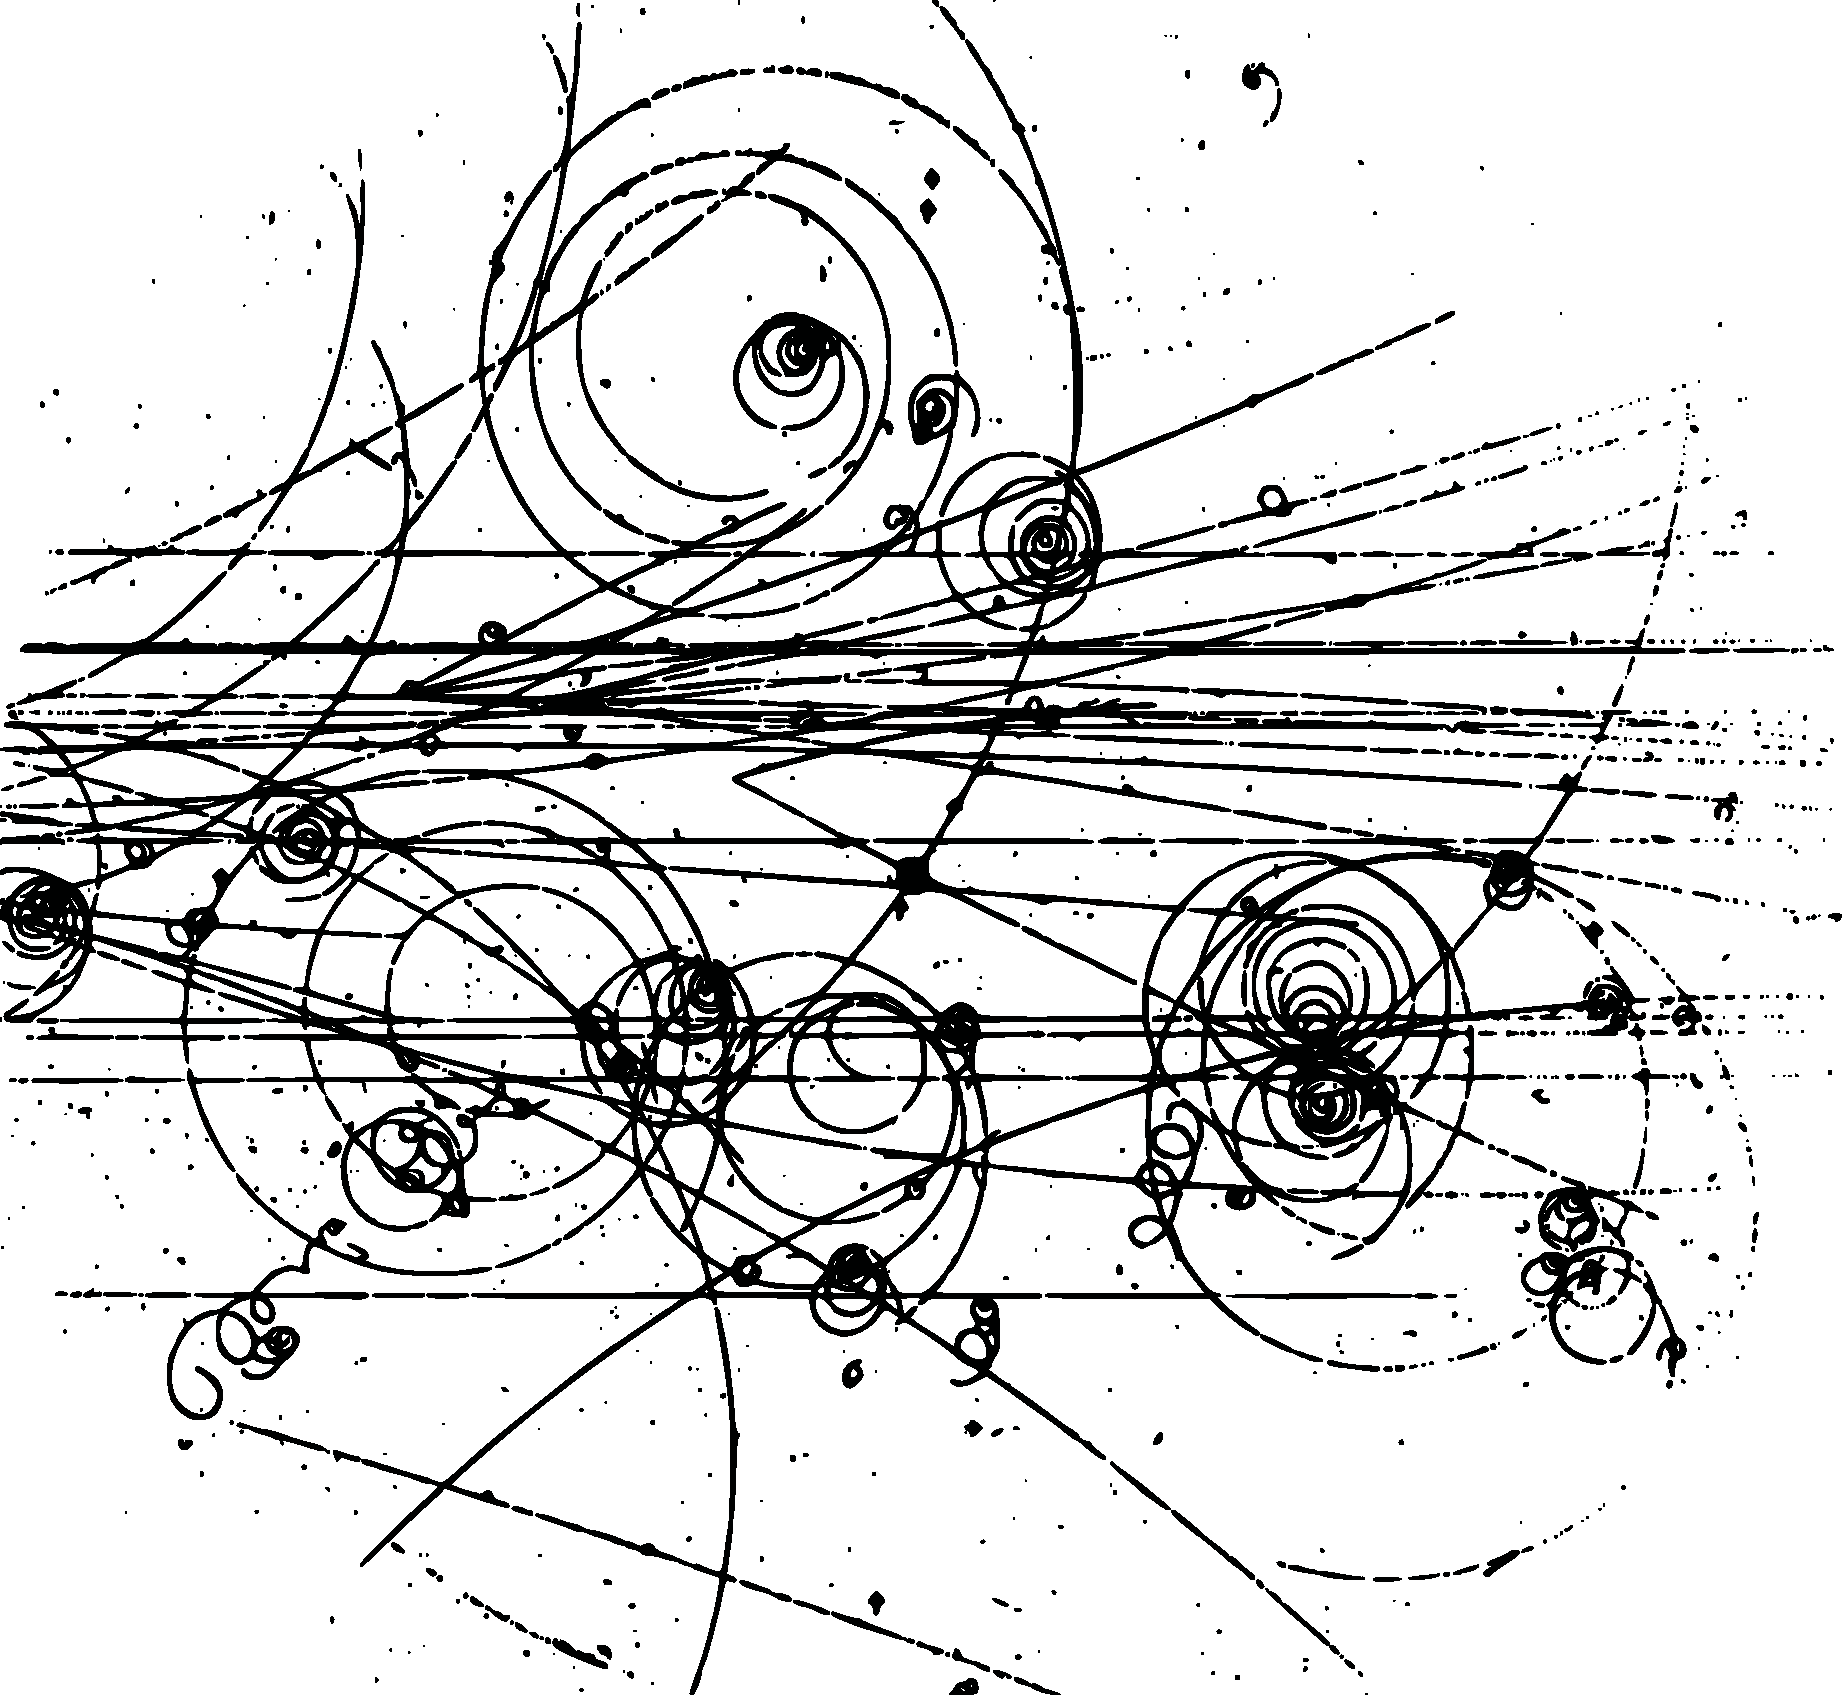
\includegraphics[width=0.6\linewidth]{fig/bc_1}};
%\end{tikzpicture}

\vspace{10cm}
{\huge DOKTORSKA DISERTACIJA}



\vfill

{\hfill \large Matic Lubej}

\vspace{1cm}
{\large 2018}

\cleardoublepage

\end{center}
\end{otherlanguage}

%%% NASLOVNA STRAN V ANGLESKEM JEZIKU
\pagenumbering{roman}
\pagestyle{empty}
\begin{center}


\includegraphics{fig/logo2}

{\large UNIVERSITY OF LJUBLJANA\\
FACULTY OF MATHEMATICS AND PHYSICS\\
DEPARTMENT OF PHYSICS\\}

\vspace{5cm}

{\Large Matic Lubej\\}

\vspace{10mm}

{\bf \Large Measurement of the $\bm{B^+ \to K^+K^-\ell^+\nu_\ell}$ Decay with the Belle Detector\\}
\vspace{5mm}
{\large Doctoral thesis}\\

\vfill

{\large ADVISER: Assist. Prof. Dr. An\v ze Zupanc\\
%COADVISER: Ime in priimek\\
}

\vspace{2cm}
{\large Ljubljana, 2018}

\end{center}


%%% NASLOVNA STRAN V SLOVENSKEM JEZIKU

\cleardoublepage
\begin{otherlanguage}{slovene}
\begin{center}


\includegraphics{fig/logo2}

{\large UNIVERZA V LJUBLJANI\\
FAKULTETA ZA MATEMATIKO IN FIZIKO\\
ODDELEK ZA FIZIKO\\}

\vspace{5cm}

{\Large Matic Lubej\\}

\vspace{10mm}

{\bf \Large Meritev razpada $\bm{B^+ \to K^+K^-\ell^+\nu_\ell}$ z detektorjem Belle\\}
\vspace{5mm}
{\large Doktorska disertacija}\\

\vfill

{\large MENTOR: doc. dr. An\v ze Zupanc\\
%SOMENTOR$\backslash$-ICA: naziv, Ime in priimek\\
}



\vspace{2cm}

{\large Ljubljana, 2018}

\end{center}


%%% ZAHVALA (NEOBVEZNO)

\cleardoublepage

\pagestyle{plain}
\vfill
\chapter*{Zahvala}
Zahvala
\pagestyle{empty}

%%% IZVLECEK

\cleardoublepage
\chapter*{Izvle"cek}
V Disertaciji predstavljamo meritev razvejitvenega razmerja ne-"carobnega semileptonskega razpada \decayb. Meritev je bila opravljena na vzorcu podatkov, ki ustreza integrirani luminoznosti $710\e{fb^{-1}}$, zbranim z detektorjem Belle na asimetri"cnem trkalniku delcev $e^+e^-$ KEKB v mestu Tsukuba na Japonskem. V delu predstavimo rezultate, ki so bili pridobljeni s konverzijo B2BII. To je prva meritev tega razpada, kjer izmerimo razvejitveno razmerje $\mathcal{B}(B^+ \to K^+ K^- \ell^+ \nu) = (3.04 \pm 0.51 \pm {}^{+0.67}_{-0.66})\E{-5}$. S signifikanco $5.9\sigma$ ta meritev "steje kot prvo odkritje razpada.\\
\vspace{1cm}\\
{{\bf Klju"cne besede}:}
\begin{itemize}
	\item detektor Belle
	\item mezoni $B$
	\item semileptonski razpadi
	\item razvejitveno razmerje
\end{itemize}
\vspace{1cm}
{{\bf PACS}:}
\begin{itemize}
	\item 11.30.Er Konjugacija naboja, parnost, obrat "casa in ostale diskretne simetrije
	\item 13.20.-v Leptonski, semileptonski in radiativni razpadi mezonov
	\item 13.20.He Razpadi mezonov s kvarkom $b$
	\item 14.40.Nd Mezoni s kvarkom $b$ ($|B|>0$) 
\end{itemize}
\end{otherlanguage}

\pagestyle{empty}

%%% ABSTRACT
\cleardoublepage
\pagestyle{plain}
\chapter*{Abstract}
We present the branching fraction measurement of the charmless semileptonic decay \decayb. The measurement has been performed on a data sample corresponding to $710\e{fb^{-1}}$ of integrated luminosity, collected with the Belle detector at the KEKB asymmetric-energy $e^+e^-$ collider in Tsukuba, Japan. We present the results obtained with the B2BII data format converter. This is the first measurement of the decay, where we obtain the branching fraction of $\mathcal{B}(B^+ \to K^+ K^- \ell^+ \nu) = (3.04 \pm 0.51 \pm {}^{+0.67}_{-0.66})\E{-5}$. With the fit significance of $5.9\sigma$, this measurement counts as the first discovery of the decay.\\
\vspace{1cm}\\
{{\bf Keywords}:} 
\begin{itemize}
	\item Belle detector
	\item $B$ mesons
	\item semileptonic decays
	\item branching fraction
	\item inclusive tagging
	\item untagged
	\item rest of event
\end{itemize}
\vspace{1cm}
{{\bf PACS}:}
\begin{itemize}
	\item 11.30.Er Charge conjugation, parity, time reversal, and other discrete symmetries
	\item 13.20.-v Leptonic, semileptonic, and radiative decays of mesons
	\item 13.20.He Decays of bottom mesons 
	\item 14.40.Nd Bottom mesons ($|B|>0$) 
\end{itemize}

\pagestyle{empty}

%%% KAZALO
\tableofcontents
\pagestyle{plain}
